\section{Method} \label{sec:method}

The overarching goal of this study is to develop an accurate and transferable methodology for regional theoretical wave resource assessment. The proposed methodology for conducting regional theoretical wave energy resource assessments that eliminates double counting of the wave resource that might occur by not considering wave direction and includes all sources of wave energy that are legitimately a portion of the region's resource. Specifically,

\begin{enumerate}
    \item This methodology recommends IEC TS-101 standards for numerical model setup, configuration, and validation. In addition to the IEC requirements, the model must also be configured to output the source terms, so that the `local resource' (defined below) can be computed.
    
    \item The total wave resource is defined as the sum of the remote and local resource (Figure \ref{fig:diagram:west-eez}). To our knowledge, this is the first work to define and propose including the local resource in the total resource estimate. 

    \item Based on Article 56 of the U.N. Law of the Sea — which states that ``in the exclusive economic zone, the coastal State has sovereign rights [to] the production of energy from the water, currents and winds'', we propose that national resource assessments should utilize the exclusive economic zone (EEZ) as the domain over which wave energy resource totals are calculated (United Nations General Assembly 1982). At the same time, we believe that the resource that is very distant from shore is, practically speaking, beyond the reach of wave technologies that exist today. For this reason we also estimate an 'inner-shelf' resource that indicates the wave energy that is technically and practically available for delivery to terrestrial markets in the foreseeable future.
    
\end{enumerate}

\begin{figure}[ht]
\centering
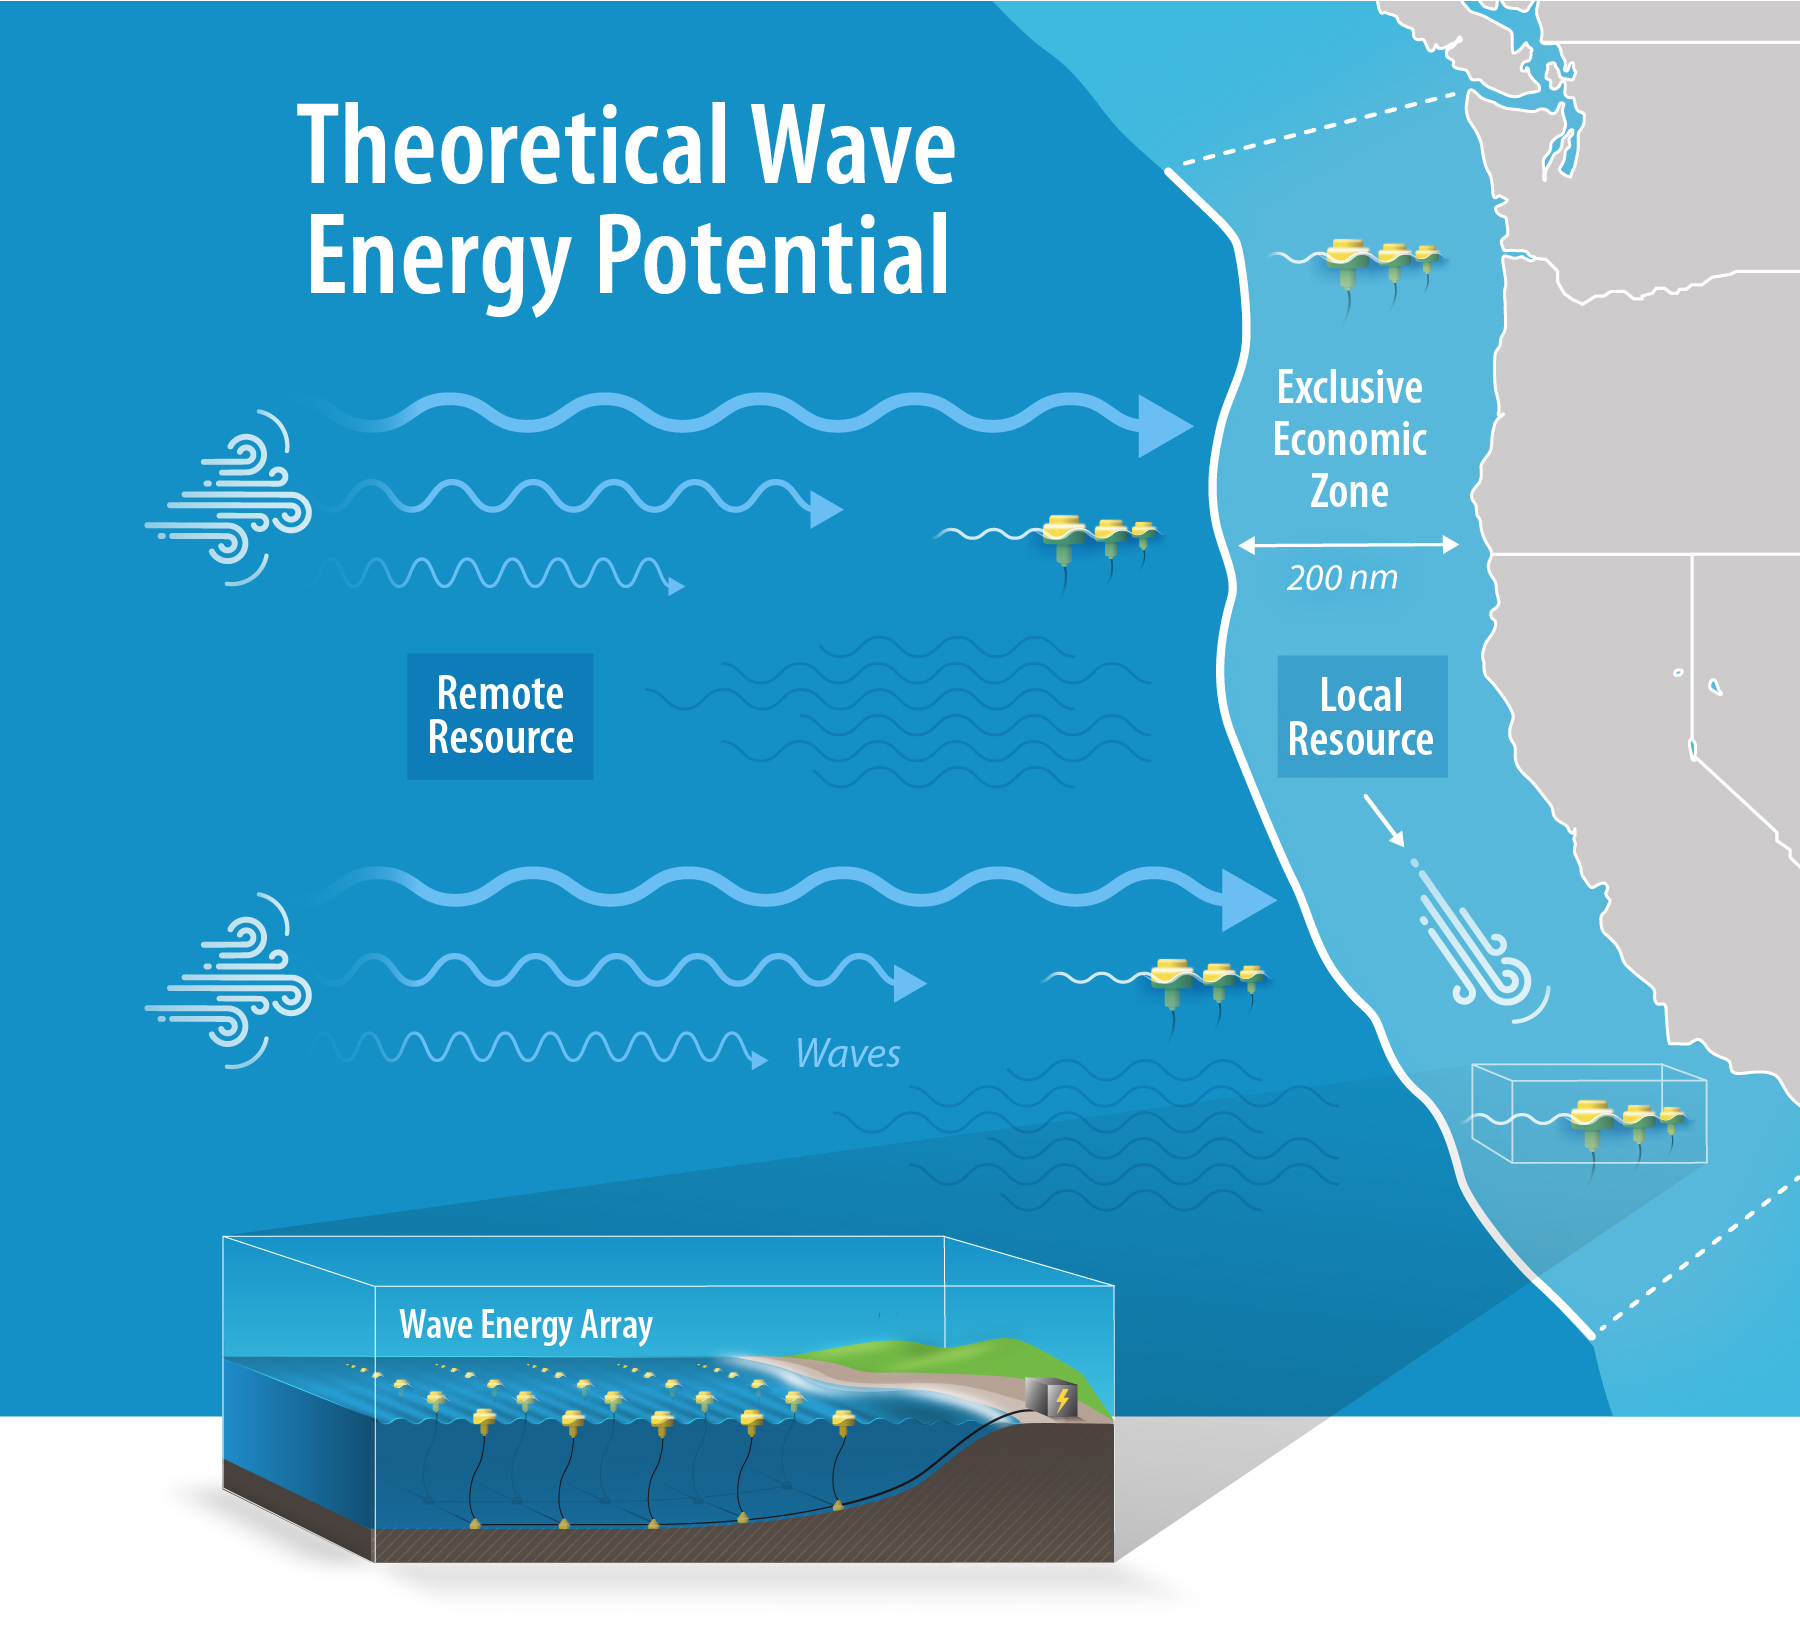
\includegraphics[width=\linewidth]{../../fig/NREL-WaveGraphic_v06.png}
\caption{A diagram depicting the U.S. West Coast's wave energy resource. The remote resource is dominated by low-frequency waves due to the preferential decay of higher-frequency waves. The local resource is defined as wave energy generated by winds within the domain of interest. The inset shows a schematic of a hypothetical wave array.}
\label{fig:diagram:west-eez}
\end{figure}

\subsection{Numerical Model} \label{sec:method:model}

Wave resource assessments use wave model `hindcasts' to estimate the history of the wave field over the region(s) of interest, and resource estimates are computed from the output of these models \citep{internationalelectrotechnicalcommissionPart101Wave2015}. This work uses WAVEWATCH III\textregistered v5.16 spanning a 31-year period from 1 January 1980 to 31 December 2010 \citep{tolmanDistributedmemoryConceptsWave2002,tolmanwavewatch}.

WAVEWATCH III\textregistered \ (hereafter WW3) is a well established numerical model that has been implemented successfully in many previous wave resource assessments \citep[e.g.,][]{garcia-medinaWaveResourceAssessment2014,hemerRevisedAssessmentAustralia2017,yangWaveModelTest2017}.
WW3 solves the five-dimensional action balance equation:

\begin{align}
  \frac{d N}{d t} = \frac{\Src{tot}}{\sigma} = \frac{1}{\sigma}\left ( \Src{in} + \Src{ds} + \Src{brk} + \Src{nl} + \Src{bot} \right )
  \label{eqn:actionbalance}
\end{align}
where $N(t,x,y,\sigma,\theta) \equiv D/\sigma$ is the wave action, $D$ is the variance spectrum, $t$ is time, $x$ and $y$ are the spatial coordinates, $\sigma$ is the radian frequency, and $\theta$ is the direction of wave propagation.
The wave action is conserved in the absence of sinks and sources of energy, their combined effect is represented as $\Src{tot}$. The present implementation of the model does not include the effects of wave reflection (e.g., at the shoreline), or of currents.

In this study we implement the ``ST4'' physics package option in WW3 to simulate energy input due to wind ($\Src{in}$) and energy dissipation due to whitecapping ($\Src{ds}$) \citep{ardhuinObservationSwellDissipation2009}.
The wind forcing is taken from NOAA's Climate Forecast System Reanalysis (CFSR) \citep{sahaNCEPClimateForecast2010}. The non-linear quadruplet interactions ($\Src{nl}$) which simulate the energy transfer from high to lower frequencies due to wave interactions are modeled with the Hasselmann and Hasselmann (\citeyear{hasselmannComputationsParameterizationsNonlinear1985}) formulation. Bottom friction ($\Src{bot}$) and depth induced wave breaking ($\Src{brk}$) are modeled with the JONSWAP Hasselmann etal. \citeyear{hasselmannMeasurementsWindwaveGrowth1973} and Battjes and Janssen \citeyear{battjesEnergyLossSetup1978} models, respectively. Finally, the effect of sea ice is considered by using a time varying mask based on the ice coverage fields from CFSR. Default parameters are used for all formulations. The wave spectrum is discretized with 24 equally spaced bins in $\theta$ space and 29 logarithmically spaced frequency bins from 0.035Hz to 0.5Hz with an increment factor of 1.1.

Model grids and bathymetry come from the NOAA NCEP hindcast Phase 1 mosaic-model \citep{chawla2011wavewatch,chawla201230,chawla_validation_2013}. In this system a global model (0.5$^{\circ}$ resolution) drives regional models (10" - 4" resolution) providing complete coverage over the U.S. EEZ with higher resolution focused on shallower waters. This model configuration is aligned with the IEC TS 62600-101 requirements for a reconnaissance class resource assessment \citep{internationalelectrotechnicalcommissionPart101Wave2015}.

The model was re-implemented in hindcast mode to store directionally-resolved wave spectra and directionally-integrated source terms. These model outputs are collected along contours spaced 10 nmi apart (18.5 km) from shore to the EEZ boundary (200 nmi from shore). Data are saved at $1/6^\circ$ increments along each contour. This was done around Alaska (excluding the Arctic Coast), Atlantic Coast, Caribbean Coast (including Puerto Rico and U.S. Virgin Islands), Gulf Coast, Hawaii (excluding the Papah$\bar{\text{a}}$naumoku$\bar{\text{a}}$kea Marine National Monument), and the West Coast. 

In WW3, as it is customary in third-generation spectral wave models, the waves are computed over a specified spectral range, after the highest modeled frequency a parametric spectral tail is appended to represent the energy in the high frequencies \citep[e.g.][]{ardhuin_semiempirical_2010}. This frequency cutoff is the minimum of the highest prescribed frequency and the cutoff supported by the source term formulations. The simulations in this study are performed with the default high frequency cutoff:

\begin{align}
    f_{c} = \frac{2.5}{T_{m01}}
    \label{eqn:freqCutoff}
\end{align}

where $T_{m01}$ is the mean spectral period.

Model-data comparisons were performed at 107 in situ stations throughout the hindcast period. The stations labeled by their World Meteorological Organization identifier are shown in Figure~\ref{fig:buoyMap}. Only stations within or close to the study areas were considered. Two statistical metrics are calculated to quantify the model performance, the centered root-mean-squared difference (CRMSD):
\begin{align}
    CRMSD^{2} = \frac{1}{N} \sum_{n=1}^{N} \left[ \left(P_{n} - \overline{P} \right) - \left(M_{n} - \overline{M} \right) \right]^{2}
\end{align}

\noindent and the correlation coefficient

\begin{align}
    R = \frac{\frac{1}{N}\sum_{n=1}^{N}\left(P_{n} - \overline{P} \right) - \left(M_{n} - \overline{M} \right)}{\sigma_{P} \sigma_{M}};
\end{align}

\noindent where $N$ is the number of observations, $P$ is the predicted quantity, $M$ is the measured quantity, and $\sigma$ is the standard deviation; whose geometric relationship is described in \citet[][]{taylor_summarizing_2001}. These statistics computed for significant wave height are shown in Figure~\ref{fig:validationHs}. The model was found to perform well with average central root mean squared difference and correlation coefficients of 0.34 m and 0.92, respectively. The error statistics for most of the buoys show CRMSD between 0.25 and 0.5 m and linear correlation coefficients above 0.9. These errors are similar to those in the implementation the present model is based on \citep[][]{chawla_validation_2013}. 

\begin{figure}[ht]
  \centering
  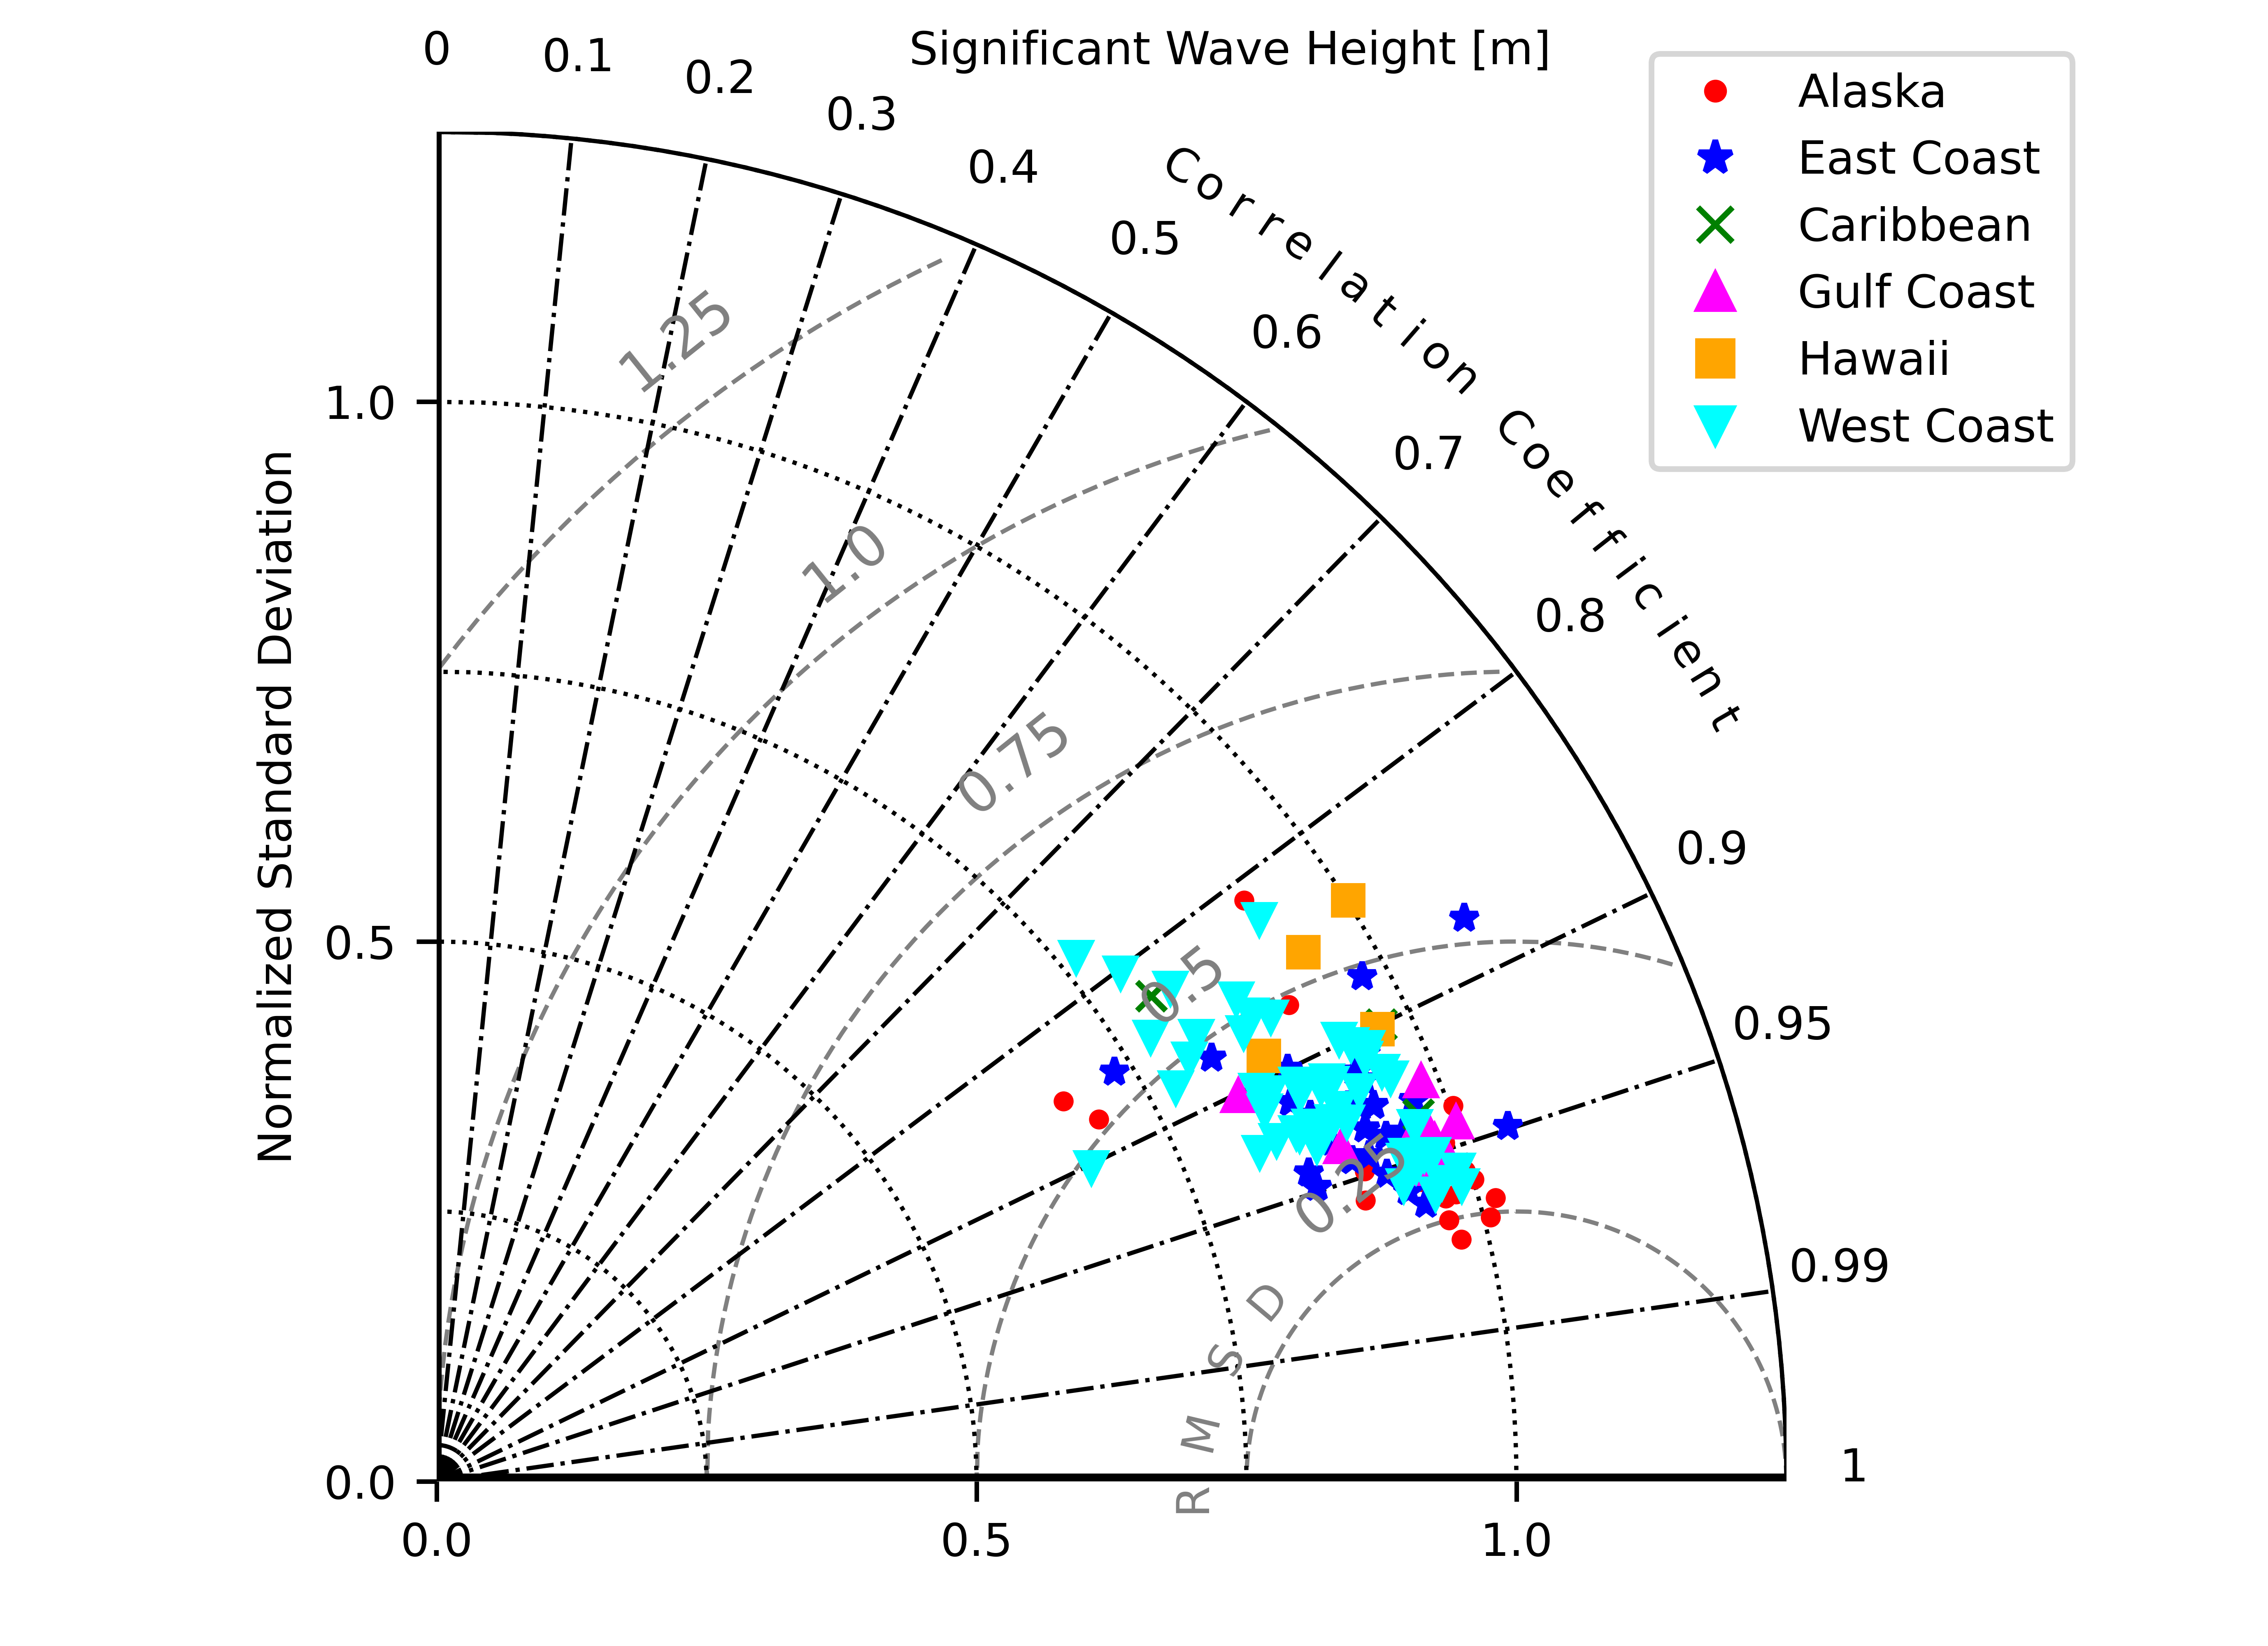
\includegraphics[width=140mm]{../../fig/taylorBasicHs.png}
  \caption{Error statistics for significant wave height.}
  \label{fig:validationHs}
\end{figure}

\subsection{The Total Resource ($R_T$) \label{sec:method:calc}}

In this work we propose that the total theoretical wave resource, $R_T$, be defined as a sum of `remote' ($R$) and `local' ($L$) components:
\begin{align}
  R_T = R_R + R_L
\end{align}
The remote resource, $R_R$, is the piece of the wave energy resource that has previously been defined as the total wave resource \citep{gunnQuantifyingGlobalWave2012,EPRIwaveresource2011}.

\subsubsection{Remote Resource ($R_{R}$)} \label{sec:method:calc:remote}

The remote resource is defined as the wave energy that propagates into the domain, and is calculated utilizing a one-way dot-product at the boundary of the domain. This approach has been used in several previous wave resource assessments \citep{gunnQuantifyingGlobalWave2012, hemerRevisedAssessmentAustralia2017, regueroGlobalWavePower2015, garcia-medinaWaveResourceAssessment2014}, and a detailed rationale is also provided in \ref{appendix:one-way-method}. 

In particular, the remote resource is computed as a line-integral of the wave energy that fluxes toward the coastline across the EEZ boundary.

\begin{align}
  R_R = \rho g \int_{\ell}\iint \delta \, c_g(f) \, \bar{D}(f,\theta) \d f \d \theta \d l
\label{eqn:RR}
\end{align}
where $\rho$ is the water density, $g$ is gravitational acceleration, $c_g(f)$ is the wave group velocity, $\ell$ is the integration contour, $D \left(f,\theta\right)$ is the wave-variance spectrum, and
the over-bar denotes a time-average of the wave-variance spectrum over the 31-year model period. The frequency integral is taken over the range where waves are actively simulated (up to $f_{c}$).

The directionality coefficient is $\delta = \cos(\theta_n - \theta)$ for waves propagating toward the coastline, and $\delta = 0$ otherwise.  $\theta_n$ is the direction normal to the contour pointing toward the shoreline. Utilizing this `one-way dot-product', is important because it minimizes the double counting found in `direction agnostic' approaches (such as EPRI 2011), and also does not erroneously subtract from the total where wave energy propagates offshore across the domain boundary \citep{nationalresearchcouncilEvaluationDepartmentEnergy2013,gunnQuantifyingGlobalWave2012}.

The integration contour ($\ell$) is composed of the segments of the U.S. EEZ that separate U.S. EEZ waters from international waters (hereafter the `EEZ boundary'; thick white line in Figure \ref{fig:diagram:west-eez}), and does not include the EEZ segments that separate one nation's EEZ from that of a neighbor \citep[]{flandersmarineinstituteMaritimeBoundariesGeodatabase2018}. This is because wave-energy that propagates across these `EEZ borders' is already included (using the methodology described here) in the resource of nations from which the waves originate, and should not be counted a second time when that energy propagates into the waters of a neighbor.

\subsubsection{Local Resource ($R_{L}$)} \label{sec:method:calc:local}
   
The local resource is the wave energy that is generated by winds within the boundary of the domain. Including it in the total is a means for accounting for the `recovery' of the wave-field inshore of a project where the remote resource might already have been harnessed.

The local resource is computed as an area-integral of the following wave source- and sink-terms:

\begin{align}
  R_L &= \rho g \int_{EEZ}\iint \left ( \bar{S}_{in} + \bar{S}_{ds} + \bar{S}_{nl} \right ) \d \theta \d f \d A
\label{eqn:RL}
\end{align}
where $dA$ is differential-area.

Note that the depth-induced wave breaking ($S_{brk}$) and bottom friction ($S_{bot}$) terms are neglected in \eqref{eqn:RL} because they close \eqref{eqn:actionbalance} by dissipating all of the energy that arrives at the shoreline. Including these terms, therefore, would be contrary to the purposes of resource assessment, because the goal is to calculate how much wave energy exists \textit{before} it dissipates at the shoreline.

It is tempting to also ignore the white-capping ($\bar{S}_{ds}$) and non-linear terms ($\bar{S}_{nl}$) — both of which are also negative across this frequency range — because this would yield a significantly larger estimate of $R_L$. Doing so, however, is scientifically questionable for three reasons. First, the spatial and temporal scales at which $S_{in}$ delivers energy to the wave field is similar to the scales at which $S_{ds}$ removes it. Second, the details of wave-generation is an active area of research, with large uncertainty associated with each term's magnitude, but their sum is well constrained as demonstrated by the performance of wave models in general \citep[e.g.][]{ardhuin_semiempirical_2010,van_vledder_source_2016}. Third, there are practical challenges to generating electricity at-scale from the high-frequency (short wavelength) portion of the spectrum where most of $S_{in}$ energy exists. Therefore, it seems prudent to include $S_{nl}$ and $S_{ds}$ in our estimate of $R_L$ in order to quantify the degree to which lower-frequency waves are generated by winds.

\subsection{The Inner-Shelf Resource ($R_I$)}

The approach above provides a scalable, comprehensive, and self-consistent methodology for quantifying the total resource that is available within a nation's EEZ. However, because the EEZ extends 200 nautical miles from shore — and given the pre-commercial state of wave energy technology — it is unrealistic to expect that all of this wave energy can be harnessed at large scale in the foreseeable future. For this reason, we find it useful to also estimate the resource that is available closer to shore.

The inner-shelf resource, $R_I$, is estimated according to \eqref{eqn:RR} with the integration contour, $\ell$, evaluated along the 10 nmi contour, rather than the EEZ boundary.  The local resource within 10 nmi of shore is small (5\% in Alaska, $<2$\% for all other regions), and so for simplicity we define $R_I$ only in terms of \eqref{eqn:RR}. 
This also suggests why most previous resource assessments have neglected the local resource — because it is only relevant when wave energy extraction reaches very large spatial scales. As an example, consider fetch limited wave growth under a constant 10 m/s wind in deep water. Following \citet{donelan1980similarity} it will require 50 km of fetch for waves to have a modest wave flux of 1.5 kW/m. 

Admittedly, 10-nautical miles is somewhat arbitrary, but it has the advantage of being easy to estimate. So long as a one-way dot-product is used, and assuming that 10-nautical miles is far enough offshore that depth-induced wave energy dissipation is small, the results should not be sensitive to the chosen boundary. In other words, 10-nautical miles seems to be a convenient distance from shore such that: a) $R_L$ is small inshore of 10-nautical miles, and b) it is far enough offshore that water depths are typically too large for mooring.

\subsection{The Potential Resource ($R_P$)}

Because the source terms in \eqref{eqn:RL} depend on the sea-state and the sea-state depends on energy extracted ``up-wave'', there is ambiguity in estimating $R_L$ related to where and when wave energy is extracted by WECs. To address this, we calculate two estimates of $R_L$. The first, `natural local resource' ($R_L$) is calculated from the source-terms where waves from the global domain propagate freely throughout the EEZ. The second, `potential local resource' ($R_{L_*}$) is calculated from the source-terms when no wave energy propagates across the EEZ boundary. In other words, this is a `lake case' that only contains waves generated by winds within the regional domain. The potential resource is then defined as:

\begin{align}
    R_P = R_{L_*} - R_L
\end{align}

This `potential resource' can be interpreted as the additional energy that might be available in the local resource if the entirety of the remote resource, $R_R$, were extracted at the EEZ boundary. However, because accessing this energy is a long way from being technically viable we do not include it in $R_T$, and instead document it here as a way to indicate a maximum upper bound on wave energy potential. 

\subsection{Summary of methodology}

There is an inherent tension throughout the field of resource assessment (i.e., beyond just wave energy) between including all possible sources, and being realistic about what is accessible. For this reason, the IEC — like other renewable energy sectors — has defined terminology that helps clarify some of the underlying assumptions that are made \citep[][]{internationalelectrotechnicalcommissionPartTerminologyEdition2020}. We propose that $R_T$ is the most appropriate estimate of a nation's theoretical resource, and that adding $R_P$ to $R_{R}$ provides a maximum upper bound. We believe that the approach proposed in this study is as optimistic as possible without being unrealistic — which is exactly the intent of theoretical resource assessment.  On the other hand, for assessments of a nation's `technical' or `practical' resource, we suggest that — given the current state of wave energy technology — $R_I$ is the most appropriate quantity on which to base those assessments.

%%% Local Variables:
%%% TeX-master: "wave_res"
%%% End:
